%! TEX root = ../thesis_pres.tex

\section{Introduction}
\label{sec:introduction}


\begin{frame}
  \frametitle{Introduction}

  \begin{columns}
    \begin{column}{.48\textwidth}

      \begin{itemize}
        \item New major roles for MAVs
        \item Operations in GPS denied environments
        \item Semi-direct Visual Odometry~\cite{Forster2014}
          \begin{itemize}
            \item 300 frames per second
          \end{itemize}
      \end{itemize}

    \end{column}

    \begin{column}{.48\textwidth}
        %\centering
        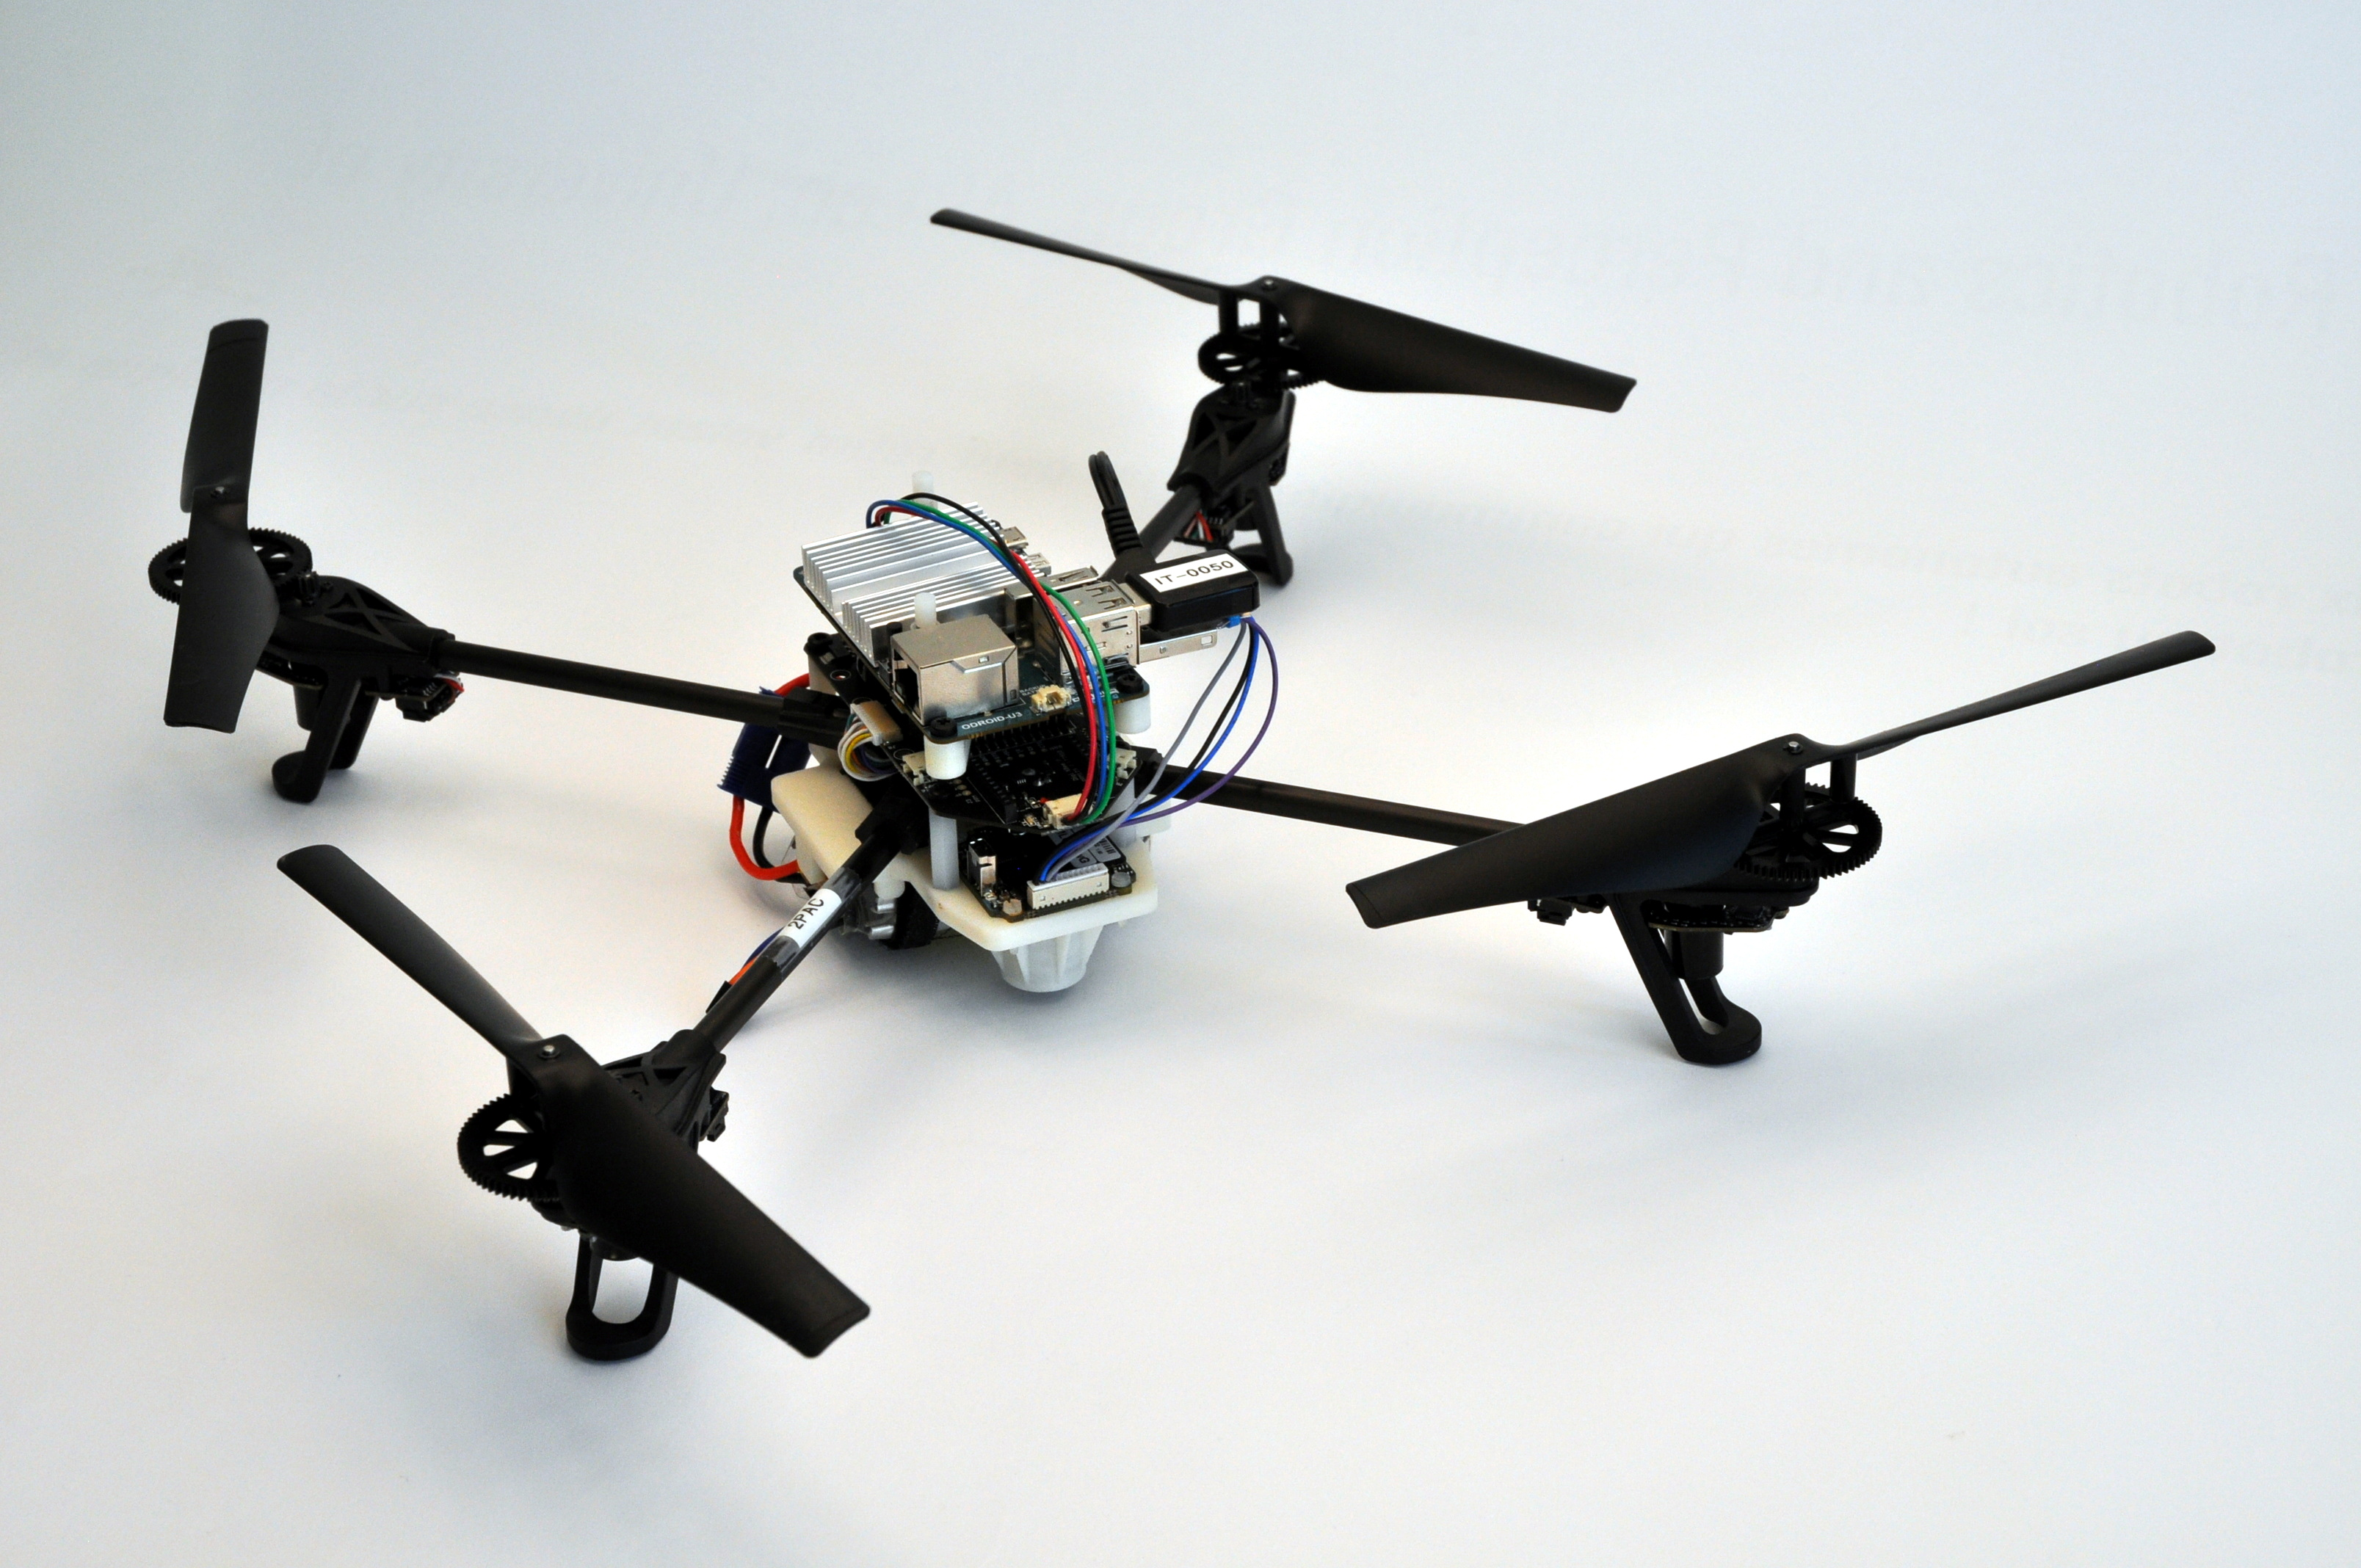
\includegraphics[width=1\linewidth]{quadro_img.jpg}
    \end{column}
  \end{columns}

\end{frame}


\begin{frame}[t]{Problem}

  \begin{columns}
    \begin{column}{0.7\textwidth}
      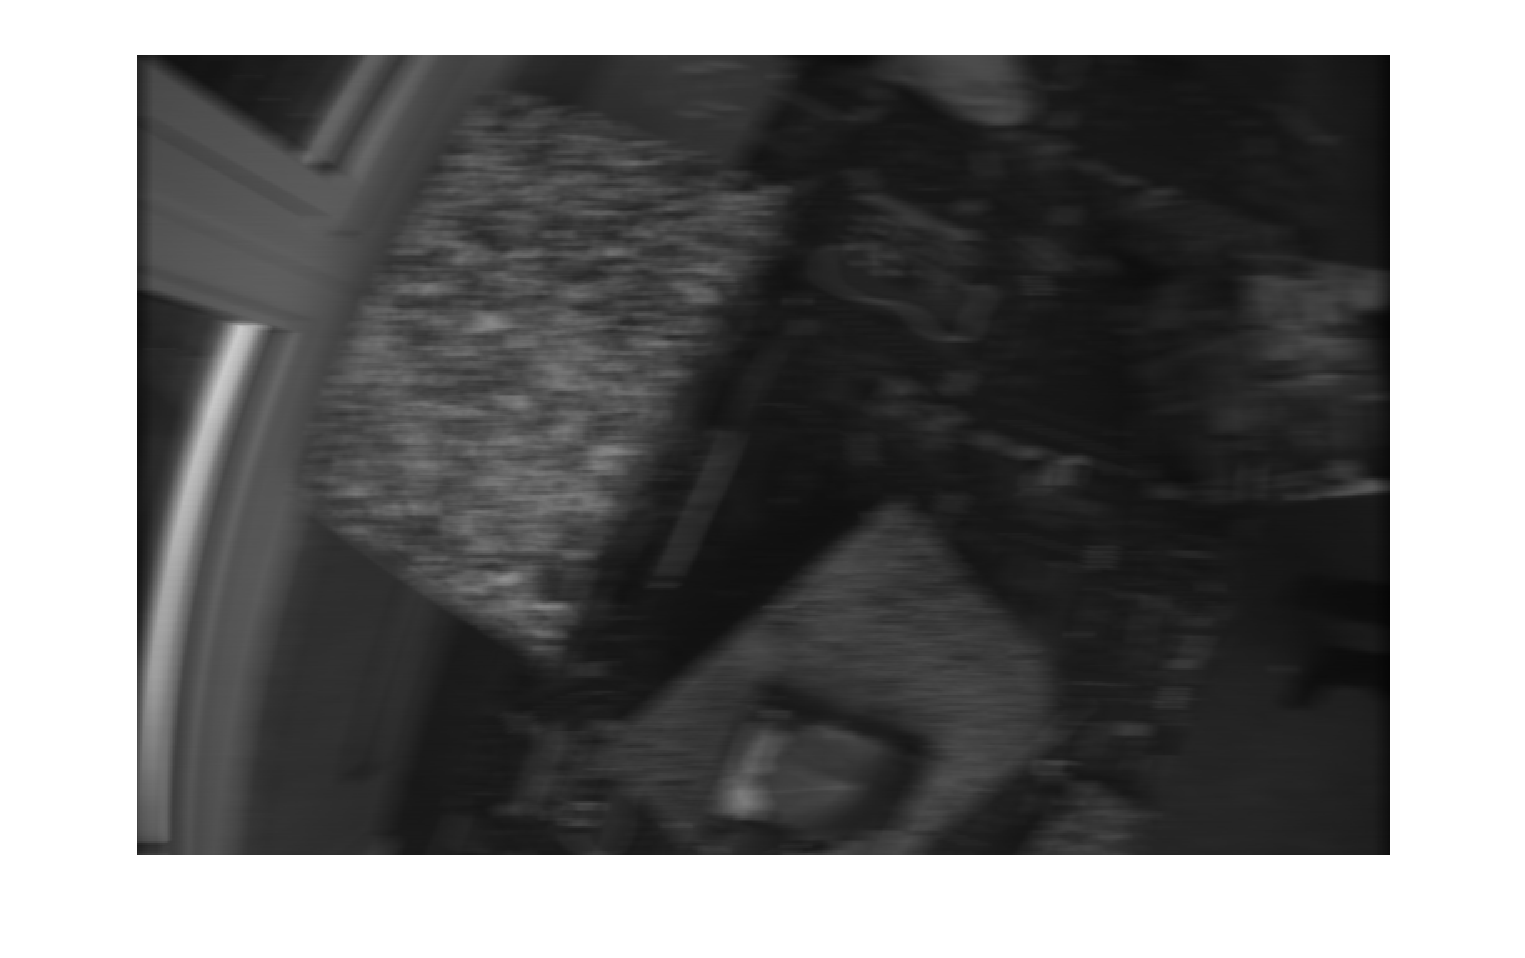
\includegraphics[width=1\linewidth]{motion_blur.eps}
      
    \end{column}

    \begin{column}{0.3\textwidth}

      \begin{block}{Tracking failure}
        \begin{itemize}
          \item Rapid camera motions
          \item Image occlusion
          \item Motion blur
        \end{itemize}
      \end{block}

    \end{column}
  \end{columns}

  \qquad A fast and accurate relocalization method is important.
  
\end{frame}

\begin{frame}[t]{Scenario}
  \begin{itemize}
    \item Area recognition. Training stage. 
    \item Tracking is lost. Drone makes a flip.
    \item Fast 6 DoF relocalization.
      \begin{itemize}
        \item Provide the pose after relocalization
        \item SVO can accept it or not
      \end{itemize}
  \end{itemize}

  \begin{block}{Implementation}
    \begin{itemize}
      \item Independent, extendible, no dependencies from SVO
      \item Fast, C++
      \item ROS
    \end{itemize}
  \end{block}



\end{frame}

